\subsection{Methodology}


We propose a methodology to demystify GPU microarchitectural features and correlate them with microbenchmark performance.
The workflow in Figure~\ref{fig:workflow} consists of three major components: a GPU ISA encoding solver, a GPU assembler, and the meticulous benchmarks.
The sample programs in Figure~\ref{fig:workflow} are synthetic PTX files which generate specific instructions as the input of the instruction solver.
Deliberate microbenchmarks are designed in assembly to figure out the correlation between microarchitecture and performance.
%We dissemble a binary library (such as cuBLAS) to provide a high coverage of instructions to instruction solver.
%We use cuBLAS in this work since it contains nearly all needed instructions for SGEMM routine.

%\jli{describe the size of samples}
We write a simple generator to produce PTX instructions with various modifiers as the PTX samples.
% We first leverage CUDA binary tools ({\tt cuobjdump} and {\tt nvdisasm}) to disassemble {\tt cubin} generated by sample programs. 
The generated PTX files are compiled to {\tt cubin} files by {\tt PTXAS}, and
then disassembled by {\tt cuobjdump} to generate native disassembly (around 2300 instruction variants). 
The ISA encoding solver takes the disassembly {\em sass} file as the input to decode each field of 64-bit instructions.
A set of algorithms are designed to solve all fields, {\em operands}, {\em opcodes}, and {\em modifiers} of a binary instruction.
{\tt cuobjdump} and {\tt nvdisasm} are used to disassemble temporary instructions generated from the solver algorithms.
%The solver uncovers some undocumented ISA specifications,
%which is used to implement an naive assembler.
Our assembler translates every instruction field to get 64-bit binaries and then encapsulates them with an ELF header to generate an executable cubin file.
% which can be used by CUDA driver APIs.
%\jli{describe microbenchmark and size: one sentence}
In the benchmarking workflow (dashed arrows in Figure~\ref{fig:workflow}), assembly microbenchmarks are tuned to explore GPU microarchitectural features such as register bank, instruction throughput, control codes, and load/store width.
% In the end, the tuning process will lead to some practical observations on the correlation between microarchitecture and performance.


\begin{figure}[htbp]
\begin{center}
    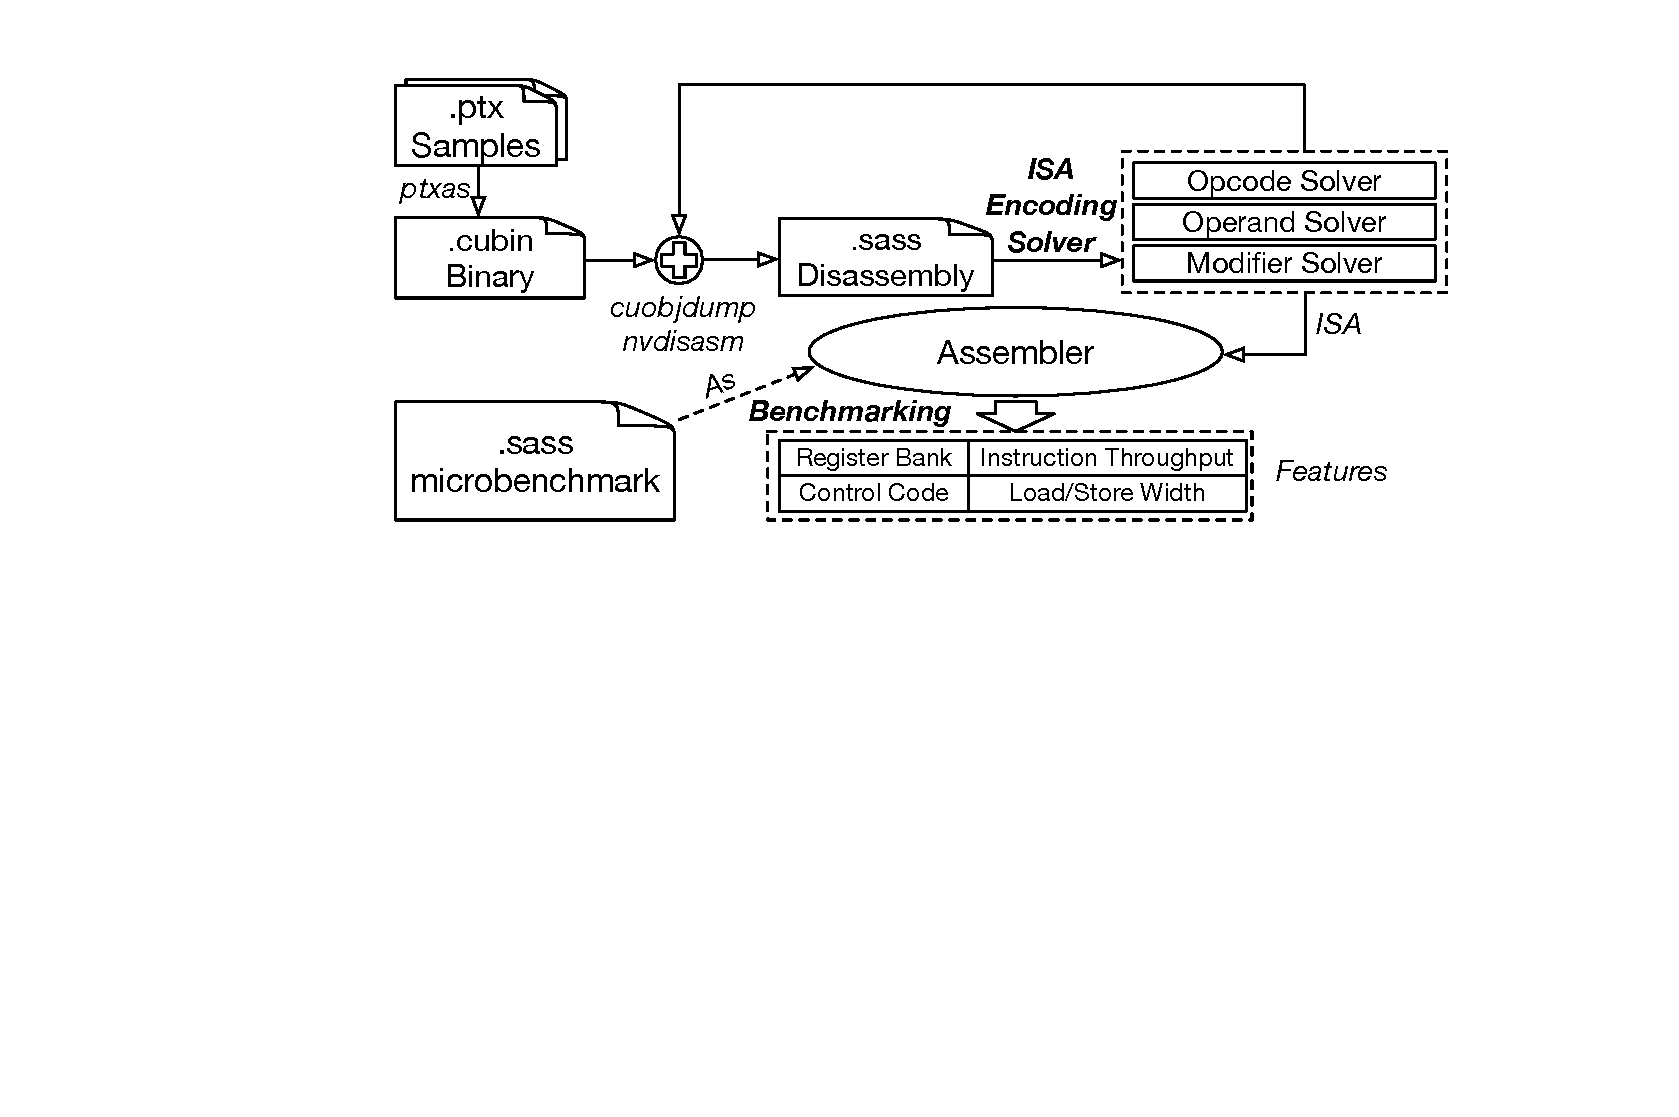
\includegraphics[scale=0.4]{methodology_new}
\caption{\small A schematic diagram of demystifying GPU microarchitectural features by leveraging CUDA binary tools. The solid arrows
    represent the workflow of instruction solver while the dashed ones represent benchmarking to find out the correlation between microarchitectures and performance.}
\label{fig:workflow}
\end{center}
\end{figure}
